\clearpage
\section{FIELDS AND FORMS}
If $p\in\F{R}^n$, the set of all pairs $(p,v)$, for $v\in \F{R}^n$, is denoted $\F{R}^n p$, and 
called the \textbf{tangent space}\index{Tangent space} of $\F{R}^n$ at $p$. This set is made into a vector space in 
the most obvious way, by defining
\begin{align*}
    (p,v) + (p,w) & = (p, v+w) \\
    a\cdot (p, v) & = (p, av)
\end{align*}

A vector $v\in\F{R}^n$ is often pictured as an arrow from 0 to $v$; the
vector $(p,v)\in\F{R}^n$ may be pictured (Figure \ref{Fig 4-1}) as an arrow
with the same direction and length, but with initial point $p$.

\begin{figure}[H]
    \centering
    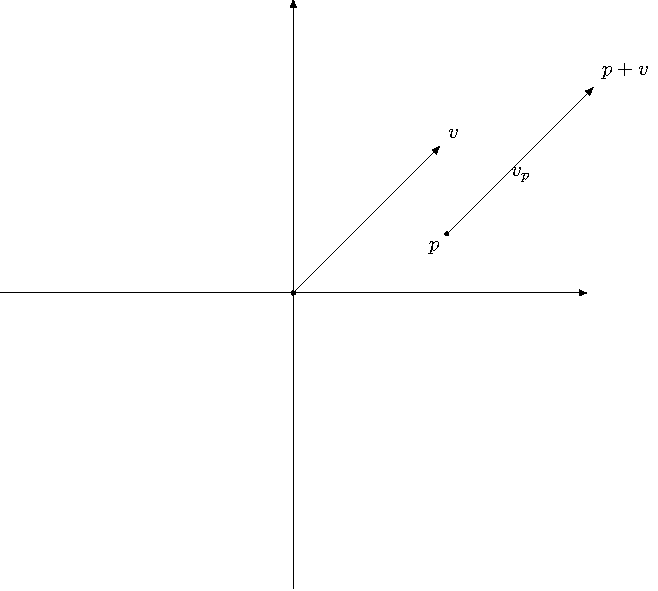
\includegraphics[width=.75\linewidth]{./pics/Fig4-1.pdf}
    \caption{}
    \label{Fig 4-1}
\end{figure}

This arrow goes from $p$ to the point $p + v$, and we therefore
define $p + v$ to be the \textbf{end point}\index{End point} of $(p,v)$.
We will usually write $(p,v)$ as $v_p$ (read: the vector $v$ at $p$).

The vector space $\F{R}^n_p$ is so closely allied to $\F{R}^n$ that many
of the structures on $\F{R}^n$ have analogues on $\F{R}^n_p$. 
In particular the \textbf{usual inner product}\index{Inner product!usual} $\langle \cdot\rangle_p$ for $\F{R}^n_p$ 
is defined by $\langle v_p, w_p\rangle_p = \langle v,w\rangle$, 
and the \textbf{usual orientation}\index{Orientation!usual} for $\F{R}^n_p$ is $[(e_1)_p, \cdots, (en)_p]$. 

Any operation which is possible in a vector space may be
performed in each $\F{R}^n_p$, and most of this section is merely an
elaboration of this theme. About the simplest operation in a vector space is the 
selection of a vector from it. If such a selection is made in each $\F{R}^n_p$, we 
obtain a \textbf{vector field}\index{Vector field} (Figure \ref{Fig 4-2}). To be precise, a vector field is a 
function $F$ such that $F(p)\in \F{R}^n_p$ for each $p\in\F{R}^n$. For each 
$p$ there are numbers $F^1(p), \cdots,F^n(p)$ such that
\begin{align*}
    F(p) = F^1(p)\cdot (e_1)_p + \cdots + F^n(p)\cdot (e_n)_p
\end{align*}

\begin{figure}[!htb]
    \centering
    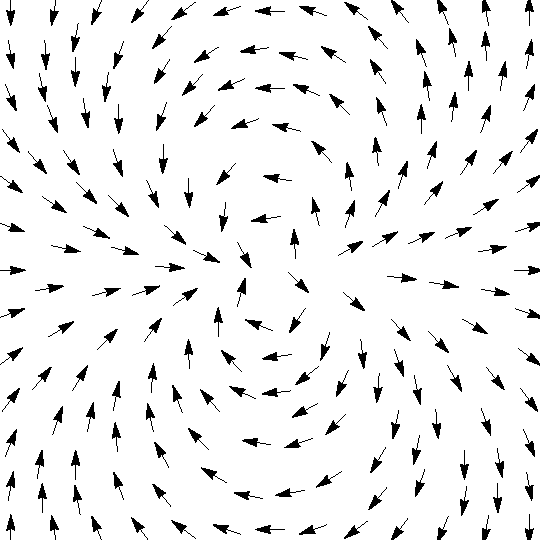
\includegraphics[width=.4\linewidth, angle=90]{./pics/Fig4-2-(1).pdf}
    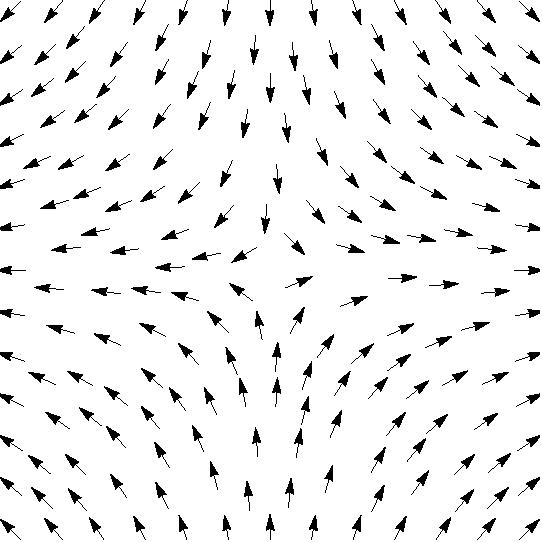
\includegraphics[width=.4\linewidth, angle=90]{./pics/Fig4-2-(2).pdf}
    \caption{}
    \label{Fig 4-2}
\end{figure}

We thus obtain $n$ \textbf{component functions}\index{Component function}\index{Function!component} $F^i:\F{R}^n\to \F{R}^n$.
The vector field $F$ is called continuous\index{Vector field!continuous}\index{Continuous vector field}, differentiable\index{Vector field!differentiable}\index{Differentiable vector field}, etc., if the
functions $F^i$ are. Similar definitions can be made for a vector
field\index{Vector field!on a manifold!continuous} defined only on an open subset of $\F{R}^n$. Operations on
vectors yield operations on vector fields when applied at each
point separately. For example, if $F$ and $G$ are vector fields
and $f$ is a function, we define
\begin{align*}
    (F+G)(p) & = F(p) + G(p) \\
    \langle F, G\rangle(p) & = \langle F(p), G(p)\rangle \\
    (f\cdot F)(p) & = f(p)\cdot F(p)
\end{align*}

If $F_1,\cdots,F_{n-1}$ are vector filed on $\F{R}^n$, then we can 
similarly define 
\begin{align*}
    (F_1\times\cdots\times F_{n-1})(p) = F_1(p)\times\cdots\times F_{n-1}(p)
\end{align*}

Certain other definitions are standard and useful. We define the \textbf{divergence}\index{Divergence of a field}, 
$\div F$ of $F$, as $\sum_{i=1}^{n}{D_iF^i}$. If we introduce the formal symbolism
\begin{align*}
    \nabla = \sum_{i=1}^{n}{D_i\cdot e_i}
\end{align*}

we can write, symbolically, $\div F = \langle \nabla, F\rangle$. If $n=3$
we write, in conformity with this symbolism,
\begin{align*}
    (\nabla\times F)(p) 
    & = (D_2F^3 - D_3F^2)(p)\cdot (e_1)_p \\
    & + (D_3F^1 - D_1F^3)(p)\cdot (e_2)_p \\
    & + (D_1F^2 - D_2F^1)(p)\cdot (e_3)_p
\end{align*}

The vector field $\nabla\times F$ is called $\curl F$.\index{Curl}
The names ``divergence'' and ``curl'' are derived from physical considerations
which are explained at the end of this book. 

Many similar considerations may be applied to a function $\omega$ with 
$\omega(p)\in \Lambda^k(\F{R}^n_p)$; such that a function is called a 
$k$\textbf{-form} on $\F{R}^n$ or simply a \textbf{differential form}\index{Differential form}.
If $\varphi_1(p),\cdots,\varphi_n(p)$ is the dual basis to $(e_1)_p,\cdots,(e_n)_p$, then 
\begin{align*}
    \omega(p) = \sum_{i_1<\cdots<i_k}{\omega_{i_1,\cdots,i_k}(p)\cdot \varphi_{i_1}(p)\wedge\cdots\wedge\varphi_{i_k}(p)}
\end{align*}

for certain functions $\omega_{i_1},\cdots,\omega_{i_k}$; the form $\omega$ 
is called continuous\index{Continuous differential form}\index{Differential form!continuous}, differentiable\index{Differential form!differentiable}\index{Differentiable differential form}, etc., if these functions are.
We shall usually assume tacitly that forms and vector fields are differentiable,
and ``differentiable'' will henceforth mean ``$C^\infty$''\index{Differentiable $=C^\infty$}; this is a
simplifying assumption that eliminates the need for counting
how many times a function is differentiated in a proof.
The sum $\omega+\eta$, product $f \cdot \omega$, and \textbf{wedge product}\index{Wedge product}
$\omega\wedge\eta$ are defined in the obvious way. A function $f$ is 
considered to be a 0-form and $f\cdot \omega$ is also written $f\wedge\omega$.

If $f:\F{R}^n\to \F{R}^n$ is differentiable, then $\R{D}f(p)\in\Lambda^1(\F{R}^n)$. 
By a minor modification we therefore obtian a 1-form $\dd f$, defined by 
\begin{align*}
    \dd f(p)(v_p) = \R{D}f(p)(v)
\end{align*}

Let us consider in particular the 1-forms $\dd \pi^i$. It is customary to let $x^i$ denote the 
\textit{function} $\pi^i$. (On $\F{R}^3$ we often denote $x^1,x^2,\text{ and }x^3$ by $x, y,\text{ and } z$).
This standard \textbf{notation}\index{Notation} has obvious disadvantages but it allows many classical results to be expressed by 
formula of equality appearance. Since $\dd x^i(p)(v_p) =\dd \pi^i(p)(v_p) = \R{D}\pi^i(p)(v) = v^i$, we 
see that $\dd x^1(p),\cdots,\dd x^n(p)$ is just the dual basis to $(e_1)_p,\cdots,(e_n)_p$. Thus
every $k$-form $\omega$ can be written
\begin{align*}
    \omega = \sum_{i_1<\cdots<i_k}^{}{\omega_{i_1,\cdots,i_k}\cdot \dd x^{i_1}\wedge\cdots\wedge\dd x^{i_k}}
\end{align*}

The expression for $\dd f$ is of particular interest.

\begin{theorem}
    If $f:\F{R}^n\to \F{R}$ is differentiable, then 
    \begin{align*}
        \dd f = \R{D}_1 f\cdot \dd x^1 + \cdots + \R{D}_nf\cdot \dd x^n
    \end{align*} 

    In classical notation,
    \begin{align*}
        \dd f = \frac{\partial f}{\partial x^1}\cdot \dd x^1 + \cdots + \frac{\partial f}{\partial x^n}\cdot \dd x^n
    \end{align*}
\end{theorem}

\begin{proof}
    \begin{align*}
        \dd f(p)(v_p) 
            & = \R{D}f(p)(v) 
            = \sum_{i=1}^{n}{v^i\cdot \R{D}_i f(p)} \\
            & = \sum_{i=1}^{n}{\dd x^i(p)(v_p)\cdot \R{D}_i f(p)}
    \end{align*}
\end{proof}


If we consider now a differentiable function $f:\F{R}^n\to \F{R}^m$, 
have a linear transformation $\R{D}f(p):\F{R}^n\to \F{R}^m$. Another 
minor modification therefore produces a linear transformation $f_*:\F{R}^n_p\to \F{R}^n_{f(p)}$
defined by 
\begin{align*}
    f_*(v_p) = \R{D}f(p)(v)_{f(p)}
\end{align*}

This linear transformation induces a linear transformation $f^*:\Lambda^k(\F{R}^m_{f(p)})\to \Lambda^k(\F{R}^n_p)$.
If $\omega$ is a $k$-form on $\F{R}^m$ we can therefore define a $k$-form $f^*\omega$ on $\F{R}^n$ by
$(f^*\omega)(p) = f^*(\omega(f(p)))$. Recall this means that if $v_1,\cdots,v_k\in\F{R}^n_p$, then we have 
$f^*\omega(p)(v_1,\cdots,v_k) = \omega(f(p))(f_*(v_1), \cdots, f_*(v_k))$. As an antidote to the abstractness
of these definitions, we present a theorem, summarizing the important properties of $f^*$, which allows explicit 
calculations of $f^*\omega$.

\begin{theorem}
    \begin{enumerate}[label=\upshape{(\arabic*)}]
        \item $f^*(\dd x^i) = \sum_{j=1}^{n}{\R{D}_if^i\cdot \dd x^i} = \sum_{j=1}^{n}{\frac{\partial f^i}{\partial x^j}\dd x^j}$
        \item $f^*(\omega_1+\omega_2) = f^*(\omega_1) + f^*(\omega_2)$
        \item $f^*(g\cdot \omega) = (g\circ f)\cdot f^*\omega$
        \item $f^*(\omega\wedge\eta) = f^*\omega\wedge f^*\eta$
    \end{enumerate}
\end{theorem}

\begin{proof}
  \begin{align*}
      \text{(1)}\qquad f^*(\dd x^i)(p)&(v_p)
        = \dd x^i(f(p))(f_*(v_p)) \\
      =\; & \dd x^i(f(p))\biggl(\sum_{j=1}^{n}{v^j\cdot \R{D}_jf^1(p)}, \cdots, \sum_{j=1}^{n}{v^j\cdot \R{D}_jf^m(p)}\biggr)_{f(p)} \\
      =\; & \sum_{j=1}^{n}{v^j\cdot \R{D}_jf^i(p)}\\
      =\; & \sum_{j=1}^{n}{\R{D}_jf^i(p)\cdot \dd x^j(p)(v_p)}
  \end{align*}

  The proof of (2), (3) and (4) are left to the reader.
\end{proof}

By repeatedly applying Theorem 4-8 we have, for example,
\begin{align*}
    f^*(P\dd x^1 \wedge \dd x^2 + Q\dd x^2 \wedge \dd x^3)
    & = (P\circ f)\left[f^*(\dd x^1)\wedge f^*(\dd x^2)\right]\\
    & + (Q\circ f)\left[f^*(\dd x^2)\wedge f^*(\dd x^3)\right]
\end{align*}

The expression obtained by expanding out each $f^*(\dd x^i)$ is quite
complicated. (It is helpful to remember, however, that we have 
$\dd x^i\wedge\dd x^i = (-1)\dd x^i\wedge\dd x^i = 0$)
In one special case it will be worth our while to make an explicit evaluation.

\begin{theorem}
    If $f:\F{R}^n\to \F{R}^n$ is differentiable, then 
    \begin{align*}
        f^*(h\dd x^1 \wedge \cdots \wedge \dd x^n) 
        = 
        (h\circ f)(\det f') \dd x^1\wedge \cdots \wedge \dd x^n
    \end{align*}
\end{theorem}

\begin{proof}
    Since 
    \begin{align*}
        f^*(h\dd x^1\wedge\cdots\wedge\dd x^n) 
        = (h\circ f)f^*(\dd x^1\wedge\cdots\wedge \dd x^n)
    \end{align*}

    it suffices to show that 
    \begin{align*}
        f^*(\dd x^1\wedge\cdots\wedge\dd x^n) = \det f'\cdot \dd x^1\wedge\cdots\wedge\dd x^n
    \end{align*}

    Let $p\in \F{R}^n$ and let $A=(a_{ij})$ be the matrix of $f'(p)$. Here, and whenever 
    convenient and not confusing, we shall use omit ``p'' in $\dd x^1\wedge\cdots\wedge\dd x^n$, etc.
    Then 
    \begin{align*}
        f^*(\dd x^1\wedge\cdots & \wedge\dd x^n)(e_1, \cdots, e_n)\\
        & = \dd x^1\wedge \cdots \wedge \dd x^n (f_*(e_1), \cdots, f_*(e_n)) \\
        & = \dd x^1\wedge \cdots \wedge \dd x^n \left(\sum_{i=1}^{n}a_{i1}e_i, \cdots, \sum_{i=1}^{n}a_{in}e_i\right) \\
        & = \det(a_{ij})\cdot \dd x^1\wedge \cdots \wedge \dd x^n(e_1, \cdots, e_n) \\
    \end{align*}

    by Theorem 4-6.
\end{proof}

An important construction associated with forms is a gen-
eralization of the operator d which changes 0-forms into
1-forms. If 
\begin{align*}
    \omega = \sum_{i_1<\cdots<i_k}^{}{\omega_{i_1,\cdots,i_k}\cdot \dd x^{i_1}\wedge\cdots\wedge\dd x^{i_k}}
\end{align*}

we define a $(k+1)$-form $\dd\omega$, the \textbf{dififerential}\index{Differential} of $\omega$, by 
\begin{align*}
    \dd\omega 
    & = \sum_{i_1<\cdots<i_k}^{}{\dd\omega_{i_1,\cdots,i_k}\wedge\dd x^{i_1}\wedge\cdots\wedge\dd x^{i_k}}\\
    & = \sum_{i_1<\cdots<i_k}^{}{\sum_{\alpha=1}^{n}{\R{D}_\alpha(\omega_{i_1,\cdots,i_k})\cdot \dd x^\alpha\wedge\dd x^{i_1}\wedge\cdots\wedge\dd x^{i_k}}}
\end{align*}

\begin{theorem}
    \begin{enumerate}[label=\upshape{(\arabic*)}]
        \item $\dd (\omega+\eta) = \dd\omega + \dd\eta$
        \item If $\omega$ is a $k$-form and $\eta$ is an $l$-form, then
            \begin{align*}
                \dd(\omega\wedge\eta) = \dd\omega\wedge\eta + (-1)^k\omega\wedge\dd\eta
            \end{align*}
        \item $\dd(\dd \omega) = 0$. Briefly, $\dd^2 = 0$.%\footnote[1]{Note that this is also called Poincar\'e Lemma}
        \item If $\omega$ is a $k$-form on $\F{R}^m$ and $f:\F{R}^n\to \F{R}^m$ is 
            differentiable, then $f^*(\dd\omega) = \dd(f^*\omega)$.
    \end{enumerate}
\end{theorem}

\begin{proof}
    \begin{enumerate}[label=\upshape{(\arabic*)}]
        \item Left to the reader.
        \item The formula is true if $\omega = \dd x^{i_1}\wedge\cdots\wedge\dd x^{i_k}$ and 
            $\eta = \dd x^{j_1}\wedge\cdots\wedge\dd x^{j_l}$, since all terms vanish. The formula 
            is easily checked when $\omega$ and $\eta$ are 0-form. The general formula may be derived from (1)
            and two observations.
        \item Since 
            \begin{align*}
                \dd\omega
                = \sum_{i_1<\cdots<i_k}^{}{\sum_{\alpha=1}^{n}{\R{D}_\alpha(\omega_{i_1,\cdots,i_k})\cdot \dd x^\alpha\wedge\dd x^{i_1}\wedge\cdots\wedge\dd x^{i_k}}}
            \end{align*} 

            we have 
            \begin{align*}
                \dd(\dd\omega)
                = \sum_{i_1<\cdots<i_k}^{}{\sum_{\alpha=1}^{n}{\sum_{\beta=1}^{n} \R{D}_{\alpha,\beta}(\omega_{i_1,\cdots,i_k})\dd x^\alpha\wedge\dd x^\beta\wedge\dd x^{i_1}\wedge\cdots\wedge\dd x^{i_k}}}
            \end{align*}

            In this sum the terms 
            \begin{align*}
                \R{D}_{\alpha,\beta}(\omega_{i_1,\cdots,i_k})\dd x^\beta\wedge\dd x^\alpha\wedge\dd x^{i_1}\wedge\cdots\wedge\dd x^{i_k}
            \end{align*}
            
            and 
            \begin{align*}
                \R{D}_{\beta,\alpha}(\omega_{i_1,\cdots,i_k})\dd x^\beta\wedge\dd x^\beta\wedge\dd x^{i_1}\wedge\cdots\wedge\dd x^{i_k}
            \end{align*}

            cancel in pairs.
        \item This is clear if $\omega$ is a 0-form. Suppose, induetively, that
            (4) is true when $\omega$ is a $k$-form. It suffices to prove (4) for
            a $(k + 1)$-form of the type $w\wedge \dd x^i$. We have 
            \begin{align*}
                f^*(\dd(\omega\wedge\dd x^i))
                & = f^*(\dd\omega\wedge\dd x^i + (-1)^k\omega\wedge\dd(\dd x^i)) \\
                & = f^*(\dd\omega\wedge \dd x^i) \\
                & = \dd(f^*\omega)\wedge f^*(\dd x^i) \text{\qquad by (2) and (3)} \\
                & = \dd(f^*(\omega\wedge\dd x^i))
            \end{align*}
    \end{enumerate}
\end{proof}

A form $\omega$ is \textbf{closed}\index{Closed differential form}\index{Differential form!closed} if $\dd\omega = 0$ and \textbf{exact}\index{Exact differential form}\index{Differential form!exact} if $\omega=\dd\eta$,
for some $\eta$. Theorem 4-10 show that exact from is closed, and it is natural to ask whether,
conversely, every closed form is exact. If $\omega$ is the 1-form $P\dd x + Q\dd y$ on $\F{R}^2$, 
then 
\begin{align*}
    \dd\omega
    & = (\R{D}_1P\dd x + \R{D}_2P\dd y)\wedge\dd x + (\R{D}_1Q\dd x + \R{D}_2Q\dd y)\wedge\dd y \\
    & = (\R{D}_1Q - \R{D}_2P)\dd x\wedge\dd y
\end{align*}

Thus, if $\dd\omega=0$, then $\R{D}_1Q = \R{D}_2P$. Problem 2-21 and 3-34 show that there is 
a 0-form $f$ such that $\omega=\dd f=\R{D}_1f\dd x+ \R{D}_2f\dd y$. If $\omega$ defined only 
on a subset of $\F{R}^3$, however, such a function may not exsit. The classical example is the 
form 
\begin{align*}
    \omega = \frac{-y}{x^2+y^2}\dd x + \frac{x}{x^2+y^2}\dd y
\end{align*}

defined on $\F{R}^2-\{0\}$. This form is usually denoted $\dd\theta$ (where $\theta$ is defined in Problem 3-41),
since (Problem 4-21) it equals $\dd\theta$ on the set $\{(x,y):x<0\text{ or } x\ge 0\text{ and }y\neq 0\}$,
where $\theta$ is defined. Note, however, that $\theta$ cannot be defined continuously on all of $\F{R}^2-\{0\}$.
If $\omega=\dd f$ for some function $f:\F{R}^2-\{0\}\to 0\to \F{R}$, then $\R{D}_1f = \R{D}_2\theta$ and 
$\R{D}_2f = \R{D}_2\theta$, so $f=\theta + \text{constant}$, showing that such $f$ cannot exsit.

Suppose that $\omega=\sum_{i=1}^n\omega_i\dd x^i$ is a 1-form on $\F{R}^n$ and $\omega$ happens to equal 
$\dd f=\sum_{i=1}^{n}{\R{D}_if\cdot \dd x^i}$. We can clearly assume that $f(0)=0$. As in Problem 2-35, we have 
\begin{align*}
    f(x) 
    & = \int_{0}^{1}{\frac{\partial \dd }{\partial \dd t }f(tx) \;\dd t}
        = \int_{0}^{1}{\sum_{i=1}^{n}{\R{D}_i f(tx)\cdot x^i \;\dd t}} \\
    & = \sum_{i=1}^{n}{x^i\int_{0}^{1}{\omega_i f(tx)\;\dd t}}
\end{align*}

This suggests that in order to find $f$, given $\omega$, we consider the
function $I_\omega$, defined by 
\begin{align*}
    I\omega(x)=\int_0^1\sum_{i=1}^n\omega_i(tx)\cdot x^i\dd t
\end{align*}

Note that the definition of $I_\omega$ makes sense if $\omega$ is defined only
on an open set $A\subset \F{R}^n$ with the property that whenever
$x\in A$, the line segment from 0 to xis contained in $A$; such
an open set is called \textbf{star-shaped}\index{Star-shaped} with respect to 0 (Figure \ref{Fig 4-3}).
A somewhat involved calculation shows that (on a star-shaped open set) 
we have $\omega = \dd(I\omega)$ provided that $\omega$ satisfies the 
necessary condition $\dd\omega = 0$. The calculation, as well
as the definition of $I\omega$, may be generalized considerably:

\begin{figure}[!htb]
    \centering
    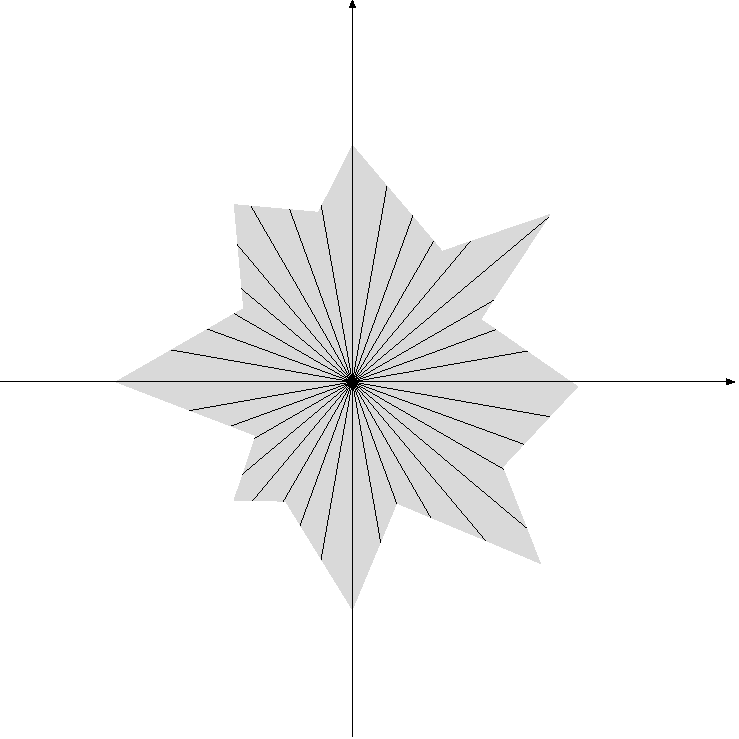
\includegraphics[width=.75\linewidth]{./pics/Fig4-3.pdf}
    \caption{}
    \label{Fig 4-3}
\end{figure}

\begin{theorem}[Poincar\'e Lemma]\index{Poincare Lemma}
    If $A\subset \F{R}^n$ is an open set star-shaped with respect to 0, 
    then every closed form on $A$ is exact.
\end{theorem}

\begin{proof}
    We will define a function $I$ from $l$-forms to $(l-I)$-
forms (for each $l$), such that $I(0) = 0$ and $\omega = I(\dd\omega) + \dd(I\omega)$
for any form $\omega$. It follows that $\omega = \dd(I\omega)$ if $\dd\omega = 0$. Let
\begin{align*}
    \omega = \sum_{i_1<\cdots<i_l}^{}{\omega_{i_1,\cdots,i_l}\dd x^{i_1}\wedge\cdots\wedge\dd x^{i_l}}
\end{align*}

Since $A$ is star-shaped we can define 
\begin{align*}
    I\omega(x) = \sum_{i_1<\cdots<i_l}^{}
        \sum_{\alpha=1}^{l}(-1)^{\alpha-1} & \left(\int_0^1t^{l-1}\omega_{i_1,\cdots,i_l}(tx)\;\dd t\right)x^{i_\alpha}\\
        & \dd x^{i_1}\wedge\cdots\wedge\widehat{\dd x^{i_\alpha}}\wedge\cdots\wedge\dd x^{i_l}
\end{align*}

(The symbol $\;\widehat{\qquad}\;$ over $\dd x^i$ indicates that it is omitted.) 
The proof that $\omega = I(\dd \omega) + \dd(I\omega)$
is an elaborate computation: We have, using Problem 3-32,
\begin{align*}
    \dd (I\omega)
    & = l\cdot\sum_{i_1<\cdots<i_l}\left(\int_0^1t^{l-1}\omega_{i_1,\ldots,i_l}(tx)\;\dd t\right)\dd x^{i_1}\wedge\cdots\wedge\dd x^{i_l} \\
    & \hspace*{1em} + \sum_{i_1<\cdots<i_l}\sum_{{\alpha}=1}^l\sum_{j=1}^n (-1)^{{\alpha}-1}\left(\int_0^1t^l\R{D}_j(\omega_{i_1,\ldots,i_l})(tx)\;\dd t\right)x^{i_\alpha} \\
    & \hspace*{9.5em} \dd x^j\wedge \dd x^{i_1}\wedge\cdots\wedge\widehat{\dd x^{i_{\alpha}}}\wedge\cdots\wedge \dd x^{i_{l}}
\end{align*}

(Explain why we have the factor $t^l$, instead of $t^{l-1}$.) We also have
\begin{align*}
    \dd\omega
    = \sum_{i_1<\cdots<i_k}^{}{\sum_{j=1}^{n}{\R{D}_j(\omega_{i_1,\cdots,i_l})\cdot \dd x^j\wedge\dd x^{i_1}\wedge\cdots\wedge\dd x^{i_l}}}
\end{align*}

Applying I to the $(l+1)$-form $\dd \omega$, we obtain
\begin{align*}
    I(\dd \omega)
    & = \sum_{i_1<\cdots<i_k}^{}\sum_{j=1}^{n}\left(\int_0^1t^l\R{D}_j(\omega_{i_1,\cdots,i_l})(tx)\;\dd t\right) x^j \dd x^{i_1}\wedge\cdots\wedge\dd x^{i_l} \\
    & \hspace*{1em} - \sum_{i_1<\cdots<i_l}\sum_{{j}=1}^n\sum_{\alpha=1}^l (-1)^{{\alpha}-1}\left(\int_0^1t^l\R{D}_j(\omega_{i_1,\ldots,i_l})(tx)\;\dd t\right)x^{i_\alpha} \\
    & \hspace*{9.5em} \dd x^j\wedge \dd x^{i_1}\wedge\cdots\wedge\widehat{\dd x^{i_{\alpha}}}\wedge\cdots\wedge \dd x^{i_{l}}
\end{align*}

Adding, the triple sums cancel, and we obtain 
\begin{align*}
    \dd(I\omega) + I(\dd\omega)
    & = \sum_{i_1<\cdots<i_l}l\cdot\left(\int_0^1t^{l-1}\omega_{i_1,\ldots,i_l}(tx)\;\dd t\right)\dd x^{i_1}\wedge\cdots\wedge\dd x^{i_l} \\
    & \hspace*{0em} + \sum_{i_1<\cdots<i_k}^{}\sum_{j=1}^{n}\left(\int_0^1t^l x^j\R{D}_j(\omega_{i_1,\cdots,i_l})(tx)\;\dd t\right) \dd x^{i_1}\wedge\cdots\wedge\dd x^{i_l} \\
    & = \sum_{i_1<\cdots<i_l}\left(\int_0^1\frac{\dd }{\dd t}\left[t^{l}\omega_{i_1,\ldots,i_l}(tx)\right]\;\dd t\right)\dd x^{i_1}\wedge\cdots\wedge\dd x^{i_l} \\
    & = \sum_{i_1<\cdots<i_l}\omega_{i_1,\ldots,i_l}(x)\dd x^{i_1}\wedge\cdots\wedge\dd x^{i_l} \\
    & = \omega
\end{align*}
\end{proof}

\begin{problems}
    \problem{
        \begin{enumerate}[label=\upshape{(\alph*)}]
            \item If $f:\F{R}^n\to\F{R}^m$ and $g:\F{R}^m\to \F{R}^p$, show that 
                $(g\circ f)_* = g_*\circ f_*$ and $(g\circ f)^* = f^*\circ g^*$.
            \item If $f,g:\F{R}^n\to \F{R}^n$, show that $\dd(f\cdot g) = f\cdot \dd g + g\cdot \dd f$.
        \end{enumerate}
    }
    \problem{
        Let $c$ be a differentiable curve\index{Curve!differentiable}\index{Differentiable curve} in $\F{R}^n$, that is, a differentiable function 
        $c:[0,1]\to \F{R}^n$. Define the \textbf{tangent vector}\index{Tangent vector}\index{Vector!tangent} $v$ of $c$ at $t$ 
        as $c_*((e_1)_t) = ((c^1)'(t), \cdots, (c^n)'(t))_{c(t)}$. If $f:\F{R}^n\to\F{R}^m$,
        show that the tangent vector to $f\circ c$ at $t$ is $f_*(v)$.
    }
    \problem{
        Let $f:\F{R}\to \F{R}$ and define $c:\F{R}\to\F{R}^2$ by $c(t) = (t,f(t))$. Show
        that the end point of the tangent vector of $c$ at $t$ lies on the
        tangent line to the graph of $f$ at $(t,f(t))$.
    }
    \problem{
        Let $c:[0,1]\to \F{R}^n$ be a curve such that $|c(t)|= 1$ for all $t$.
        Show that $c(t)_{c(t)}$ and the tangent vector to $c$ at $t$ are perpendicular.
    }
    \problem{
        If $f:\F{R}^n\to\F{R}^n$, define a vector field $\B{f}$ by $\B{f}(p) = f(p)_p\in\F{R}^n_p$.
        \begin{enumerate}[label=\upshape{(\alph*)}]
            \item Show that every vector field $F$ on $\F{R}^n$ is of the form $\B{f}$ for some $f$.
            \item Show that $\div \B{f} = \trace f'$.
        \end{enumerate}
    }
    \problem{
        If $f:\F{R}^n\to\F{R}$, define a vector field grad $f$ by 
        \begin{align*}
            (\grad f)(p) = \R{D}_1f(p)\cdot(e_1)_p + \cdots + \R{D}_nf(p)\cdot(e_n)_p 
        \end{align*}

        For obvious reasons we also write $\grad f=\nabla f$. If $\nabla f(p)=w_p$\index{Grad $f$},
        prove that $\R{D}_v f(p) = \langle v, w\rangle$ and conclude that $\nabla p$ is the 
        direction in which $f$ changing fastest at $p$.
    }
    \problem{
        If $F$ is a vector field on $\F{R}^3$, define the forms 
        \begin{align*}
            & \omega^1_p = F^1\dd x + F^2\dd y + F^3\dd z \\
            & \omega^2_p = F^2\dd y\wedge\dd z + F^2\dd z\wedge\dd z + F^3\dd x\wedge\dd y \\
        \end{align*}
        \begin{enumerate}[label=\upshape{(\alph*)}]
            \item Prove that 
                \begin{align*}
                    \dd f & = \omega^1_{\grad f} \\
                    \dd(\omega^1_p) & = \omega^2_{\curl F} \\
                    \dd(\omega^2_p) & = (\div F)\dd x \wedge \dd y \wedge \dd z
                \end{align*}
            \item Use (a) to prove that 
                \begin{align*}
                    \curl\grad f & = 0\\
                    \div\curl F  & = 0
                \end{align*}
            \item If $F$ is a vector field on a star-shaped open set $A$ and
                $\curl F = 0$, show that $F = \grad f$ for some function $f:A\to \F{R}$.
                Similarly, if $\div F = 0$, show that $F = \curl G$ for some vector
                field $G$ on $A$.
        \end{enumerate}
    }
    \problem{
        Let $f:U\to\F{R}^n$ be a differentiable function with a differentiable
        inverse $f^{-1}: f(U)\to\F{R}^n$. If every closed form on $U$ is exact, show
        that the same is true for $f(U)$. \textit{Hint:} If $d\omega = 0$ and 
        $f^*\omega = \dd\eta$. consider $(f^{-1})^*\eta$.
    }
    \problem[*]{
        Prove that on the set where $\theta$ is defined we have
        \begin{align*}
            \dd\theta = \frac{-y}{x^2+y^2}\dd x + \frac{x}{x^2+y^2}\dd y
        \end{align*}
    }
\end{problems}